%----------------------------------------------------------------------------------------
%	PACKAGES AND OTHER DOCUMENT CONFIGURATIONS
%----------------------------------------------------------------------------------------

\documentclass[paper=a4, fontsize=11pt]{scrartcl} % A4 paper and 11pt font size

% \usepackage[T1]{fontenc} % Use 8-bit encoding that has 256 glyphs
% \usepackage{fourier} % Use the Adobe Utopia font for the document - comment this line to return to the LaTeX default
% \usepackage[english]{babel} % English language/hyphenation
\usepackage{amsmath,amsfonts,amsthm,amssymb} % Math packages
\usepackage[T1]{fontenc}
\usepackage[sfdefault]{biolinum} % Option 'sfdefault' only if the base font of the document is to be sans serif
\usepackage[dvipsnames]{xcolor}
\usepackage{graphics}
\usepackage{graphicx}

\usepackage{listings}
\usepackage{xcolor}


\definecolor{codegreen}{rgb}{0,0.5,0}
\definecolor{codered}{rgb}{0.7,0.1,0.1}
\definecolor{codegray}{rgb}{0.5,0.5,0.5}
\definecolor{codepurple}{rgb}{0.58,0,0.82}
\definecolor{backcolour}{rgb}{1,1,1}

\theoremstyle{definition}
\newtheorem{definition}{Definition}

\definecolor{red}{rgb/cmyk}{0.9098,0.2471,0.2824 / 0,0.86,0.65,0}
\definecolor{citecolor}{HTML}{0071bc}
\newcommand{\colorcell}{\cellcolor{citecolor!15}}
% \definecolor{codegreen}{rgb}{0,0.6,0}
% \definecolor{codegray}{rgb}{0.5,0.5,0.5}
% \definecolor{codepurple}{rgb}{0.58,0,0.82}
% \definecolor{backcolour}{rgb}{0.95,0.95,0.92}
% \lstdefinestyle{mystyle}{
%     backgroundcolor=\color{backcolour},   
%     commentstyle=\color{codegreen},
%     keywordstyle=\color{magenta},
%     numberstyle=\tiny\color{codegray},
%     stringstyle=\color{codepurple},
%     basicstyle=\ttfamily\footnotesize,
%     breakatwhitespace=false,         
%     breaklines=true,                 
%     captionpos=b,                    
%     keepspaces=true,                 
%     numbers=left,                    
%     numbersep=5pt,                  
%     showspaces=false,                
%     showstringspaces=false,
%     showtabs=false,                  
%     tabsize=2
% }
% Use \lstset to make myStyle the global default
% \lstset{style=mystyle}

\usepackage{caption}
\usepackage{subcaption}
\usepackage{graphicx}
\usepackage{float}
\usepackage{blindtext} %for enumarations
\usepackage[]{hyperref}  %link collor

%talbe layout to the right
%\usepackage[labelfont=bf]{caption}
%\captionsetup[table]{labelsep=space,justification=raggedright,singlelinecheck=off}
%\captionsetup[figure]{labelsep=quad}

% \usepackage{sectsty} % Allows customizing section commands
% \allsectionsfont{\normalfont\scshape} % Make all sections centered, the default font and small caps

\usepackage{fancyhdr} % Custom headers and footers
\pagestyle{fancyplain} % Makes all pages in the document conform to the custom headers and footers
\fancyhead[R]{} % Empty left header
\fancyhead[C]{} % Empty center header
\fancyhead[L]{Deep Reinforcement Learning} % Course name for right header
\fancyfoot[L]{} % Empty left footer
\fancyfoot[C]{} % Empty center footer
\fancyfoot[R]{\thepage} % Page numbering for right footer
\renewcommand{\headrulewidth}{1pt} % Header underlines
\renewcommand{\footrulewidth}{1pt} % Footer underlines
\setlength{\headheight}{13.6pt} % Customize the height of the header

% \numberwithin{equation}{section} % Number equations within sections (i.e. 1.1, 1.2, 2.1, 2.2 instead of 1, 2, 3, 4)
% \numberwithin{figure}{section} % Number figures within sections (i.e. 1.1, 1.2, 2.1, 2.2 instead of 1, 2, 3, 4)
% \numberwithin{table}{section} % Number tables within sections (i.e. 1.1, 1.2, 2.1, 2.2 instead of 1, 2, 3, 4)

%\setlength\parindent{0pt} % Removes all indentation from paragraphs - comment this line for an assignment with lots of text
\newcommand{\dmcontrol}{\mono{dm\_control} }
\newcommand{\dmenv}{\mono{dm\_env} }
\newcommand{\mujoco}{\textsf{MuJoCo} }
\newcommand{\numpy}{\textsf{NumPy} }

% \setlength\parskip{4pt}

%----------------------------------------------------------------------------------------
%	TITLE SECTION
%----------------------------------------------------------------------------------------

\newcommand{\horrule}[1]{\rule{\linewidth}{#1}} % Create horizontal rule command with 1 argument of height

\title{	
\normalfont \normalsize 
\textsc{Ferdowsi University of Mashhad} \\ [25pt] % Your university, school and/or department name(s)
\horrule{0.5pt} \\[0.4cm] % Thin top horizontal rule
\huge  Project Report \\ % The assignment title
\horrule{2pt} \\[0.5cm] % Thick bottom horizontal rule
\date{}
}
\author{Zahra Niazi} % Your name



\begin{document}
%\nocite{*}
\maketitle % Print the title
\thispagestyle{empty}

\newpage
\begin{abstract}
{\noindent{\Large Abstract} }\\

In this document, a report on the idea and implementation of the article \textit{"Stabilizing Deep Q-Learning with ConvNets under Data Augmentation"} will be given. Suggestions for improving this implementation will be reviewed and finally the results of their implementation will be monitored. \\

\textbf{Key words:} Reinforcement Learning, Deep Learning, OpenAi Gym, Deepmind Control Suite, Continuous Control, physics simulation, Mujoco, Distracting Control Suite, dmc2gym

\end{abstract}

\newpage
\tableofcontents

%----------------------------------------------------------------------------------------
%	Section 1
%----------------------------------------------------------------------------------------
\newpage
\section{Preliminaries}
\subsection{dm-control\cite{tunyasuvunakool2020}}
Controlling the physical world is an essential aspect and arguably a prerequisite for achieving general intelligence. Primates, which have been engaging in two-handed manipulation for millions of years, provide the only known example of general-purpose intelligence.
In contrast to board games, language, and other symbolic domains, physical tasks possess a fundamental characteristic of continuity in terms of state, time, and action. The dynamics of physical systems adhere to second-order equations of motion, where the state is comprised of positions and velocities. Sensory signals, or observations, carry meaningful physical units and exhibit variations over corresponding timescales. These unique properties, along with their widespread occurrence and significance, distinguish control problems as a distinctive subset within the realm of general Markov Decision Processes. Notably, in many physical control tasks, there exists a fixed subset of degrees of freedom within the agent's body that can be directly manipulated, while the remaining degrees of freedom belong to the surrounding environment. These "embodied" tasks represent the central focus of \dmcontrol.

\subsubsection{Tasks}
In recent years, there has been significant advancement in the application of Reinforcement Learning (RL) to challenging problem domains, including video games. The Arcade Learning Environment (ALE) played a crucial role in facilitating these advancements by providing a standardized set of benchmarks for evaluating and comparing learning algorithms. Similarly, in the field of control and robotics, there is a need for well-designed task suites that serve as a standardized platform where different approaches can compete and new methods can emerge.
The OpenAI Gym has become a widely adopted benchmark in continuous RL, offering a collection of continuous control domains. To meet the growing demand for task suites that enable the study of algorithms related to multi-scale control, multi-task transfer, and meta-learning, various recent task suites have been introduced, such as Meta-world, SURREAL, RLbench and IKEA. These task suites aim to provide diverse environments for experimentation. Similarly, \dmcontrol offers its own set of control tasks, categorized into three distinct categories: 

\begin{description}
\item{\textbf{Control Suite}}

The DeepMind \textsf{Control Suite}, is built directly with the \mujoco wrapper, provides a set of standard benchmarks for continuous control problems. The unified reward structure offers interpretable learning curves and aggregated suite-wide performance measures. Furthermore, it emphasises high-quality, well-documented code using uniform design patterns, offering a readable, transparent and easily extensible codebase.
%
\item{\textbf{Locomotion}}

The Locomotion framework is designed to facilitate the implementation of a wide range of locomotion tasks for RL algorithms by introducing self-contained, reusable components which compose into different task variants. 
%
\item{\textbf{Manipulation}}

We also provide examples of constructing robotic manipulation tasks. These tasks involve grabbing and manipulating objects with a 3D robotic arm. The set of tasks includes examples of reaching, placing, stacking, throwing, assembly and disassembly.
The tasks are designed to be solved using a simulated 6 degree-of-freedom robotic arm based on the Kinova Jaco, though their modular design permit the use of other arms with minimal changes. 
These tasks make use of reusable components such as bricks that snap together, and provide examples of reward functions for manipulation.
Tasks can be run using vision, low-level features, or combinations of both.

\end{description}

\newpage
\subsection{The Distracting Control Suite\cite{stone2021distracting}}
Robotic systems often encounter demanding perceptual conditions, such as variations in viewpoint, lighting, and background. However, existing simulated reinforcement learning benchmarks, like DM Control, lack such complexities in visual input. Consequently, the performance of well-established methods on these benchmarks may not translate effectively to real-world scenarios. Here this limitation is addressed by expanding DM Control to include three types of visual distractions: variations in background, color, and camera pose. This augmented benchmark serves as a challenging testbed for vision-based control, and the study evaluates state-of-the-art RL algorithms within these settings. The experimental results reveal that current RL methods for vision-based control exhibit subpar performance in the presence of distractions. Furthermore, the performance deteriorates as the complexity of distractions increases, highlighting the necessity for novel approaches capable of handling the visual intricacies encountered in real-world environments. Additionally, the research findings indicate that combinations of multiple distraction types pose greater difficulties than merely aggregating their individual effects.

A significant challenge in perception is the ability to extract task-relevant information from sensory input while filtering out distractions that may introduce misleading correlations in subsequent tasks. However, DM Control lacks such distractions, as the agent is presented with a consistent camera view, fixed lighting conditions, and a static background. Since any observation change in DM Control corresponds directly to a change in a task-relevant state variable, it does not allow for the measurement or development of the capability to filter out irrelevant variations through perception.

To address this limitation, the Distracting Control Suite is introduced, which is an expansion of DM Control specifically designed with real-world robot learning in mind. This extension incorporates three distinct types of distractions: random color changes applied to all objects in the scene, random video backgrounds, and random continuous variations in camera pose. Each distraction can be implemented in a static setting, where changes occur only during episode transitions, or in a dynamic setting, where distractions change smoothly between frames. Furthermore, the difficulty of each distraction can be adjusted, ranging from barely noticeable to highly distracting. Additionally, all three types of distractions can be combined in any desired manner, allowing for arbitrary combinations of distractions.

\newpage
\subsection{DMControl Generalization Benchmark\cite{hansen2021softda}}
We assess the performance of our method on a set of tasks taken from the DeepMind Control Suite (DMControl), as well as in the domain of robotic manipulation. The DMControl Suite consists of a diverse range of challenging continuous control tasks and is widely recognized as a benchmark for vision-based RL. To measure the generalization capabilities of our method, a new benchmark called DMControl Generalization Benchmark (DMControl-GB) is introduced, which is built upon DMControl. In this benchmark, agents are trained in a fixed environment referred to as the training environment, and we evaluate their generalization performance on two distinct test distributions: (1) environments with randomized colors and (2) environments with natural videos serving as backgrounds. These test distributions represent the color hard and video easy benchmarks within DMControl-GB.

While DMControl-GB provides a solid platform for evaluating algorithm performance, our ultimate objective is to develop algorithms capable of solving real-world problems using vision-based RL. To better emulate real-world deployment scenarios, we also consider a robotic manipulation task involving a robotic arm in a simulated environment. Similar to DMControl-GB, agents are trained in a fixed environment and then evaluated in environments with randomized colors and video backgrounds. Additionally, we introduce random perturbations to camera settings, lighting conditions, and texture variations during testing to simulate real-world conditions.


%----------------------------------------------------------------------------------------
%	Section 2
%----------------------------------------------------------------------------------------

\newpage
\section{Stabilized $Q$-Value Estimation under Augmentation\cite{hansen2021stabilizing}}
Reinforcement Learning (RL) with visual observations has shown impressive success in various applications. However, the challenge lies in generalizing the learned skills to new environments, especially in high-dimensional observation spaces like images. To tackle this, researchers have explored domain randomization and data augmentation techniques to increase training data variability and promote invariant policies. Simple augmentations like cropping and translation have improved sample efficiency, but additional augmentation can decrease efficiency and lead to divergence. Balancing stability and generalization in RL requires careful trial and error, as the introduction of diverse data poses optimization challenges and risks instability, distinguishing it from supervised learning approaches.

To address these problems, \textbf{SVEA} (\textbf{S}tabilized $Q$-\textbf{V}alue \textbf{E}stimation under \textbf{A}ugmentation) is proposed. It is a simple yet effective framework for data augmentation in off-policy RL that greatly improves stability of $Q$-value estimation. 

\subsection{\textbf{Method}}
The method introduced is called SVEA: \textbf{S}tabilized $Q$-\textbf{V}alue \textbf{E}stimation under \textbf{A}ugmentation, which is a comprehensive framework for achieving visual generalization in reinforcement learning (RL) through the application of data augmentation. SVEA utilizes a novel learning approach that incorporates two distinct data streams: one with augmented data and another without augmentation. This method seamlessly integrates with any standard off-policy RL algorithm without requiring modifications to the underlying neural network that parameterizes the policy. Additionally, it does not involve additional forward passes, auxiliary tasks, or learnable parameters. While SVEA in principle does not make any assumptions about the structure of states $\mathbf{s}_{t} \in \mathcal{S}$,  this method is described within the context of image-based RL.


\subsubsection{\textbf{Architectural Overview}}
This approach utilizes common neural network architectures in off-policy RL without introducing additional learnable parameters. In this method, the neural network layers and corresponding learnable parameters of the state-action value function are divided into two sub-networks:
\begin{itemize}
    \item $f_{\theta}$ referred to as the state encoder
    \item $Q_{\theta}$ referred to as the Q-function
\end{itemize}
This subdivision allows us to predict the Q-value, $q_{t}$, for a given state-action pair $(\mathbf{s}_{t}, \mathbf{a}_{t})$ as:
\begin{center}
$q_{t} \triangleq Q_{\theta}(f_{\theta}(\mathbf{s}_{t}), \mathbf{a}_{t})$
\end{center}
Similarly, the target $Q$-value for $(\mathbf{s}_{t}, \mathbf{a}_{t})$ is defined as:
\begin{center}
$q^{\textnormal{tgt}}_{t} \triangleq r(\mathbf{s}_{t}, \mathbf{a}_{t}) + \gamma \max_{\mathbf{a}'_{t}} Q^{\textnormal{tgt}}_{\psi}(f^{^{\textnormal{tgt}}}_{\psi}(\mathbf{s}_{t+1}), \mathbf{a}')$
\end{center}
where $\gamma$ is the discount factor, and $\psi$ represents parameters defined as an exponential moving average of $\theta$. Depending on the chosen algorithm, we may also incorporate a parameterized policy, $\pi_{\theta}$, that shares the encoder parameters with $Q_{\theta}$ and selects actions $\mathbf{a}_{t} \sim \pi_{\theta}(\cdot|f_{\theta}(\mathbf{s}_{t}))$.

To avoid incorrect bootstrapping resulting from augmented data, data augmentation is strictly applied only in the estimation of Q-values for the current state, $\mathbf{s}_{t}$, and not to the successor state, $\mathbf{s}_{t+1}$, used for bootstrapping with $Q^{\text{tgt}}_{\psi}$ (and $\pi_{\theta}$ if applicable). To mitigate over-regularization during the optimization of $f_{\theta}$ and $Q_{\theta}$, we utilize a modified Q-objective that incorporates both augmented and unaugmented data.

\subsubsection{\textbf{Learning Objective}}
This method redefines the temporal difference objective to better leverage data augmentation. First, recall that $q^{\textnormal{tgt}}_{t} = r(\mathbf{s}_{t}, \mathbf{a}_{t}) + \gamma \max_{\mathbf{a}'_{t}} Q^{\textnormal{tgt}}_{\psi}(f^{^{\textnormal{tgt}}}_{\psi}(\mathbf{s}_{t+1}), \mathbf{a}')$. Instead of learning to predict $q^{\textnormal{tgt}}_{t}$ only from state $\mathbf{s}_{t}$, it is proposed to minimize a nonnegative linear combination of $\mathcal{L}_{Q}$ over two individual data streams, $\textcolor{citecolor}{\mathbf{s}_{t}}$ and $\textcolor{Fuchsia}{\mathbf{s}^{\textnormal{aug}}_{t} = \tau(\mathbf{s}_{t}, \nu),~\nu \sim \mathcal{V}}$, which is then defined as the objective
\begin{align}
    \mathcal{L}^{\textbf{SVEA}}_{Q}(\theta, \psi) & \triangleq \textcolor{citecolor}{\alpha \mathcal{L}_{Q}\left(\mathbf{s}_{t}, q^{\textnormal{tgt}}_{t}; \theta, \psi\right)} + \textcolor{Fuchsia}{\beta \mathcal{L}_{Q}\left(\mathbf{s}^{\textnormal{aug}}_{t}, q^{\textnormal{tgt}}_{t}; \theta,\psi\right)} \\
    \label{eq:new-critic-loss}
    & = \mathbb{E}_{\mathbf{s}_{t}, \mathbf{a}_{t}, \mathbf{s}_{t+1} \sim \mathcal{B}} \left[ \textcolor{citecolor}{\alpha \left\| Q_{\theta}(f_{\theta}(\mathbf{s}_{t}), \mathbf{a}_{t}) - q^{\textnormal{tgt}}_{t} \right\|^{2}_{2}} + \textcolor{Fuchsia}{\beta \left\| Q_{\theta}(f_\theta(\mathbf{s}^{\textnormal{aug}}_{t}), \mathbf{a}_{t}) - q^{\textnormal{tgt}}_{t} \right\|^{2}_{2}} \right] \,,
\end{align}
where $\textcolor{citecolor}{\alpha}, \textcolor{Fuchsia}{\beta}$ are constant coefficients that balance the ratio of the \textcolor{citecolor}{unaugmented} and \textcolor{Fuchsia}{augmented} data streams, respectively, and $q^{\textnormal{tgt}}_{t}$ is computed strictly from unaugmented data. $\mathcal{L}^{\textbf{SVEA}}_{Q}(\theta, \psi)$ serves as a \textit{data-mixing} strategy that \textbf{oversamples unaugmented data as an implicit variance reduction technique}. Data-mixing is a simple and effective technique for variance reduction that works well in tandem with the modifications proposed for bootstrapping. 
For $\alpha=\beta$, the objective in Eq. \ref{eq:new-critic-loss} can be evaluated in a single, batched forward-pass by rewriting it as:
\begin{align}
    \mathbf{g}_{t} & = \left[ \textcolor{citecolor}{\mathbf{s}_{t}}, \textcolor{Fuchsia}{\tau(\mathbf{s}_{t}, \nu)}\right]_{\textnormal{N}}
    \\
    h_{t} & = \left[ q^{\textnormal{tgt}}_{t}, q^{\textnormal{tgt}}_{t} \right]_{\textnormal{N}} \\
    \label{eq:new-critic-loss-single-forward-pass}
     \mathcal{L}^{\textbf{SVEA}}_{Q}(\theta, \psi) & = \mathbb{E}_{\mathbf{s}_{t}, \mathbf{a}_{t}, \mathbf{s}_{t+1} \sim \mathcal{B},~\nu \sim \mathcal{V}} \left[
    (\alpha + \beta) \left\| Q_{\theta}(f_\theta(\mathbf{g}_{t}), \mathbf{a}_{t}) - h_{t} \right\|^{2}_{2} \right]\,,
\end{align}

\subsection{\textbf{Setup}}The method and baselines are implemented using the Soft Actor-Critic (SAC) algorithm as the base. By default, random shift augmentation is incorporated into all methods. The base algorithm is referred to as the "unaugmented" version and we examine its stability under additional data augmentation. For all methods (when applicable), identical network architectures and hyperparameters are employed. Observations consist of stacked RGB frames, with a size of $84\times84\times3$. In the DMControl-GB and DistractingCS benchmarks, we train all methods for 500k frames and evaluate them on the same 5 tasks used in prior work. The same experimental setup is also applied to the robotic manipulation experiments.


\subsection{\textbf{Implementation Details}}
\textbf{Network architecture.} For experiments in DMControl, the network architecture from \cite{hansen2021softda} is adopted, without any changes to the architecture nor hyperparameters. The shared encoder $f_{\theta}$ is implemented as an 11-layer CNN encoder that takes a stack of RGB frames rendered at $84\times84\times3$ and outputs features of size $32\times 21 \times 21$, where $32$ is the number of channels and $21\times21$ are the dimensions of the spatial feature maps. All convolutional layers use $32$ filters and $3\times3$ kernels. The first convolutional layer uses a stride of 2, while the remaining convolutional layers use a stride of 1. Following previous work on image-based RL for DMControl tasks, the shared encoder is followed by independent linear projections for the actor and critic of the Soft Actor-Critic base algorithm used in our experiments, and the actor and critic modules each consist of three fully connected layers with hidden dimension $1024$. Training takes approximately 24 hours on a single NVIDIA V100 GPU.

%----------------------------------------------------------------------------------------
%	Section 3
%----------------------------------------------------------------------------------------

\newpage
\section{Experiments}

A comprehensive evaluation has been conducted of this method and a set of robust baselines, employing Convolutional Neural Networks (ConvNets), on tasks sourced from the DeepMind Control Suite (DMControl) and a collection of robotic manipulation tasks. DMControl provides a range of challenging and diverse continuous control tasks and is widely recognized as a benchmark for image-based RL. In order to assess the generalization capabilities of our method and the baselines, we subject them to rigorous distribution shifts from the \textbf{DMControl Generalization Benchmark} (DMControl-GB), the \textbf{Distracting Control Suite} (DistractingCS), as well as distribution shifts specific to the robotic manipulation environment. Our evaluation encompasses the analysis of \textit{sample efficiency}, \textit{asymptotic performance}, and \textit{generalization performance} of the methods across these varied scenarios.


\newpage
\subsection{\textbf{Data Augmentation in RL.}}

Figure \ref{fig:data-aug-visualization} provides a comprehensive set of samples for each of the data augmentations considered in this study: 
\begin{itemize}
    \item random \textit{shift}
    \item random convolution (denoted \textit{conv})
    \item random \textit{overlay}
    \item random \textit{cutout}
    \item Gaussian \textit{blur}
    \item random \textit{affine-jitter}
    \item random \textit{rotation}
\end{itemize}
It is emphasized that the random convolution augmentation is not a convolution operation, but rather application of a randomly initialized convolutional layer as in the original proposal.\\
As in previous work  that applies data augmentation to image-based RL, we either clip values or apply a logistic function, whichever is more appropriate, to ensure that output values remain within the $[0, 1)$ interval that unaugmented observations are normalized to. \\
Each of the considered data augmentations are applied to the \textit{walker} and \textit{cartpole} environments and are representative of the \textit{Walker, walk}, \textit{Walker, stand}, \textit{Cartpole, swingup}, and \textit{Cartpole, balance} tasks. To illustrate the diversity of augmentation parameters associated with a given transformation, we provide a total of 6 samples for each data augmentation in each of the two environments. \\

% Previous work applies augmentation to both state $\mathbf{s}^{\textnormal{aug}}_{t} = \tau(\mathbf{s}_{t}, \nu)$ and successor state $\mathbf{s}^{\textnormal{aug}}_{t+1} = \tau(\mathbf{s}_{t+1}, \nu')$ where $\nu,\nu' \sim \mathcal{V}$. 
% The application of weak augmentation, such as random shift, has been shown to improve sample efficiency without causing significant issues. However, it has been observed that strong augmentation, such as random convolution, can lead to instability and poor sample efficiency. The use of stronger and more varied augmentations, including random convolution, random overlay, and affine-jitter, has the potential to enhance generalization to a broader range of Markov Decision Processes (MDPs). Nonetheless, the naive application of wea augmentations has resulted in optimization challenges and reduced sample efficiency.

% We apply random shifts in SVEA and all baselines by default, and aim to stabilize learning under strong augmentation. As such, we refer to observations both with and without the random shift operation as \textit{unaugmented}, and instead refer to observations as \textit{augmented} after application of one of the 6 augmentations considered in our study. 

\begin{figure}[H]
    \centering
    \begin{subfigure}[b]{0.48\textwidth}
        \centering
        
\includegraphics[width=\textwidth]{figures/visualizations/grid_original.png}
        \caption{No augmentation (walker).}
        \vspace{0.1in}
    \end{subfigure}
    \begin{subfigure}[b]{0.48\textwidth}
        \centering
        
\includegraphics[width=\textwidth]{figures/visualizations/grid_cartpole_original.png}
        \caption{No augmentation (cartpole).}
        \vspace{0.1in}
    \end{subfigure}
    \begin{subfigure}[b]{0.48\textwidth}
        \centering
        
\includegraphics[width=\textwidth]{figures/visualizations/grid_shift.png}
        \caption{Random shift (walker).}
        \vspace{0.1in}
    \end{subfigure}
    \begin{subfigure}[b]{0.48\textwidth}
        \centering
        
\includegraphics[width=\textwidth]{figures/visualizations/grid_cartpole_shift.png}
        \caption{Random shift (cartpole).}
        \vspace{0.1in}
    \end{subfigure}
    \begin{subfigure}[b]{0.48\textwidth}
        \centering
        
\includegraphics[width=\textwidth]{figures/visualizations/grid_conv.png}
        \caption{Random convolution (walker).}
        \vspace{0.1in}
    \end{subfigure}
    \begin{subfigure}[b]{0.48\textwidth}
        \centering
        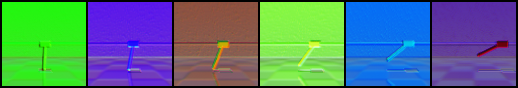
\includegraphics[width=\textwidth]{figures/visualizations/grid_cartpole_conv.png}
        \caption{Random convolution (cartpole).}
        \vspace{0.1in}
    \end{subfigure}
    \begin{subfigure}[b]{0.48\textwidth}
        \centering
        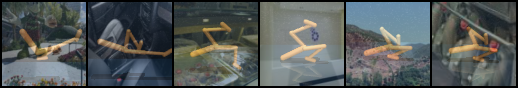
\includegraphics[width=\textwidth]{figures/visualizations/grid_overlay.png}
        \caption{Random overlay (walker).}
        \vspace{0.1in}
    \end{subfigure}
    \begin{subfigure}[b]{0.48\textwidth}
        \centering
        
\includegraphics[width=\textwidth]{figures/visualizations/grid_cartpole_overlay.png}
        \caption{Random overlay (cartpole).}
        \vspace{0.1in}
    \end{subfigure}
    \begin{subfigure}[b]{0.48\textwidth}
        \centering
        
\includegraphics[width=\textwidth]{figures/visualizations/grid_cutout.png}
        \caption{Random cutout (walker).}
        \vspace{0.1in}
    \end{subfigure}
    \begin{subfigure}[b]{0.48\textwidth}
        \centering
        
\includegraphics[width=\textwidth]{figures/visualizations/grid_cartpole_cutout.png}
        \caption{Random cutout (cartpole).}
        \vspace{0.1in}
    \end{subfigure}
    \begin{subfigure}[b]{0.48\textwidth}
        \centering
        
\includegraphics[width=\textwidth]{figures/visualizations/grid_blur.png}
        \caption{Random blur (walker).}
        \vspace{0.1in}
    \end{subfigure}
    \begin{subfigure}[b]{0.48\textwidth}
        \centering
        
\includegraphics[width=\textwidth]{figures/visualizations/grid_cartpole_blur.png}
        \caption{Random blur (cartpole).}
        \vspace{0.1in}
    \end{subfigure}
    \begin{subfigure}[b]{0.48\textwidth}
        \centering
        
\includegraphics[width=\textwidth]{figures/visualizations/grid_affinejitter.png}
        \caption{Random affine-jitter (walker).}
        \vspace{0.1in}
    \end{subfigure}
    \begin{subfigure}[b]{0.48\textwidth}
        \centering
        
\includegraphics[width=\textwidth]{figures/visualizations/grid_cartpole_affinejitter.png}
        \caption{Random affine-jitter (cartpole).}
        \vspace{0.1in}
    \end{subfigure}
    \begin{subfigure}[b]{0.48\textwidth}
        \centering
        
\includegraphics[width=\textwidth]{figures/visualizations/grid_rotation.png}
        \caption{Random rotation (walker).}
        \vspace{0.1in}
    \end{subfigure}
    \begin{subfigure}[b]{0.48\textwidth}
        \centering
        
\includegraphics[width=\textwidth]{figures/visualizations/grid_cartpole_rotation.png}
        \caption{Random rotation (cartpole).}
        \vspace{0.1in}
    \end{subfigure}
    \caption{\textbf{Data augmentation}. Visualizations of all data augmentations considered in this study. Left column contains samples from the \textit{Walker, walk} and \textit{Walker, stand} tasks, and right column contains samples from the \textit{Cartpole, swingup} and \textit{Cartpole, balance} tasks.}
    \label{fig:data-aug-visualization}
\end{figure}

The utilization of data augmentation in image-based reinforcement learning (RL) has demonstrated remarkable success by enhancing generalization and regularizing the network parameters of the Q-function and policy $\pi$. However, not all types of augmentations yield equal effectiveness. Studies show that small random crops and random shifts (image translations) significantly enhance the sample efficiency of image-based RL. However, they do not offer significant improvements in generalization to other environments. Conversely, augmentations such as random convolution exhibit substantial potential in improving generalization but are concurrently associated with instability and reduced sample efficiency. In this context, it is crucial to distinguish between \textit{weak} augmentations, such as small random translations, which enhance \textit{sample efficiency} through regularization, and \textit{strong} augmentations, such as random convolution, which improve \textit{generalization} at the cost of sample efficiency. This study specifically focuses on stabilizing deep Q-learning when applying strong data augmentation, aiming to enhance generalization capabilities.

Figure \ref{fig:dmc-svea-augs-generalization} shows training and test performance of SVEA implemented using each of the 6 data augmentations considered in this work. SVEA exhibits comparable stability and sample efficiency for all augmentations, but we find that generalization ability on the \texttt{color\_hard} benchmark of DMControl-GB is highly dependent on the choice of augmentation. Generally, we observe that augmentations such as \textit{conv}, \textit{overlay}, and \textit{affine-jitter} achieve the best generalization, but they empirically also cause the most instability in our \textit{DrQ + aug} baseline as shown in Figure \ref{fig:drq-augs-suppl}.
\begin{figure}[H]
    \centering
    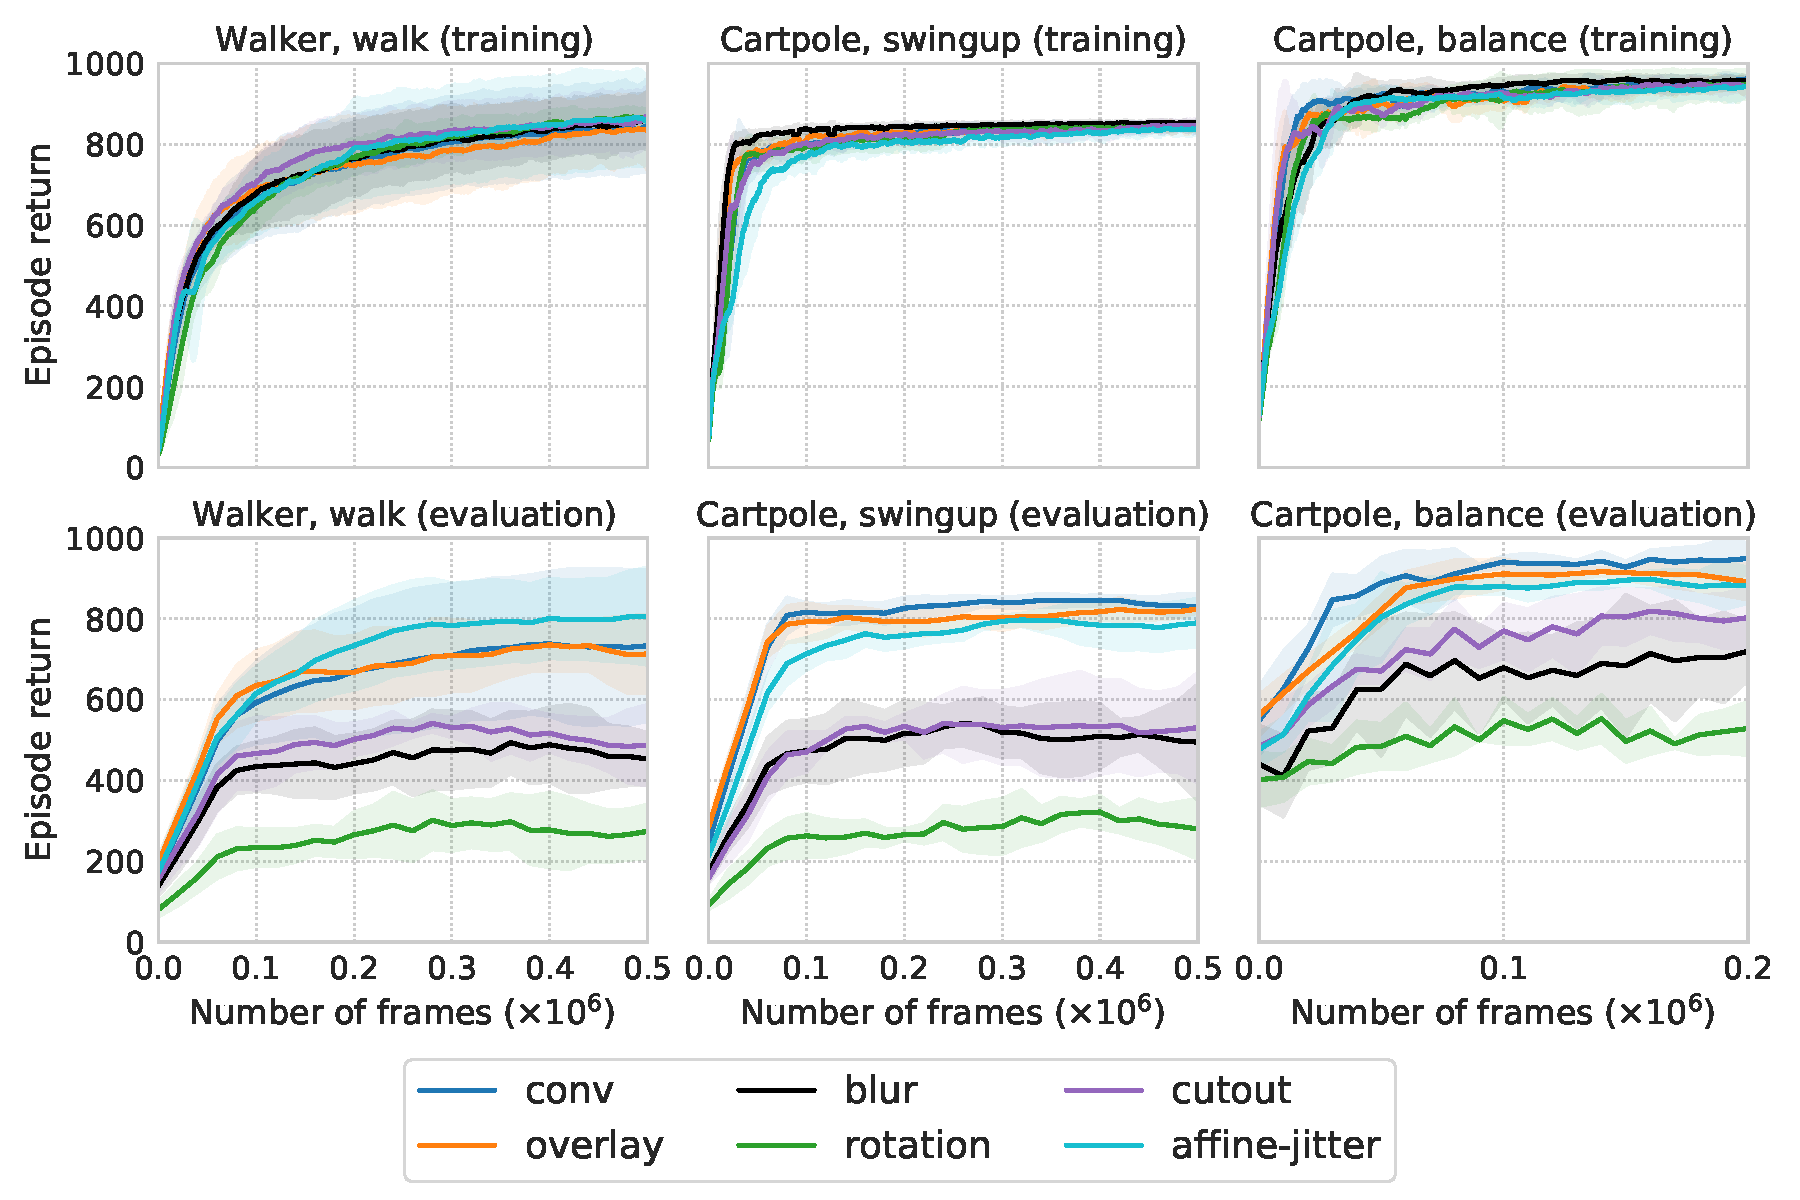
\includegraphics[width=0.64\textwidth]{figures/svea_augs_generalization.pdf}
    \vspace{-0.05in}
    \caption{\textbf{Generalization depends on the choice of data augmentation.} A comparison of SVEA implemented using each of the 6 data augmentations considered in this work (using ConvNets). SVEA exhibits comparable stability and sample efficiency for all augmentations, but generalization ability is highly dependent on the choice of augmentation. \textit{Top:} episode return on the training environment during training. \textit{Bottom:} generalization measured by episode return on the \texttt{color\_hard} benchmark of DMControl-GB. Mean of 5 seeds, shaded area is $\pm1$ std. deviation.}
    \label{fig:dmc-svea-augs-generalization}
    \vspace{-0.1in}
\end{figure}

%----------------------------------------------------------------------------------------
%	Section 4
%----------------------------------------------------------------------------------------

\newpage
\subsection*{\textbf{Stability}}

We evaluate the stability of SVEA under 6 common data augmentations; results are shown in Figure \ref{fig:dmc-augs}. SVEA is relatively unaffected by the \textbf{choice of data augmentation} and improves sample efficiency in $\mathbf{27}$ out of $\mathbf{30}$ instances. We further ablate each component of SVEA in Figure \ref{fig:dmc-conv}; we find that both components are key to SVEA's success. We observe that SVEA improves stability in all 27 instances where DrQ is impaired by data augmentation. 
\begin{figure}[H]
    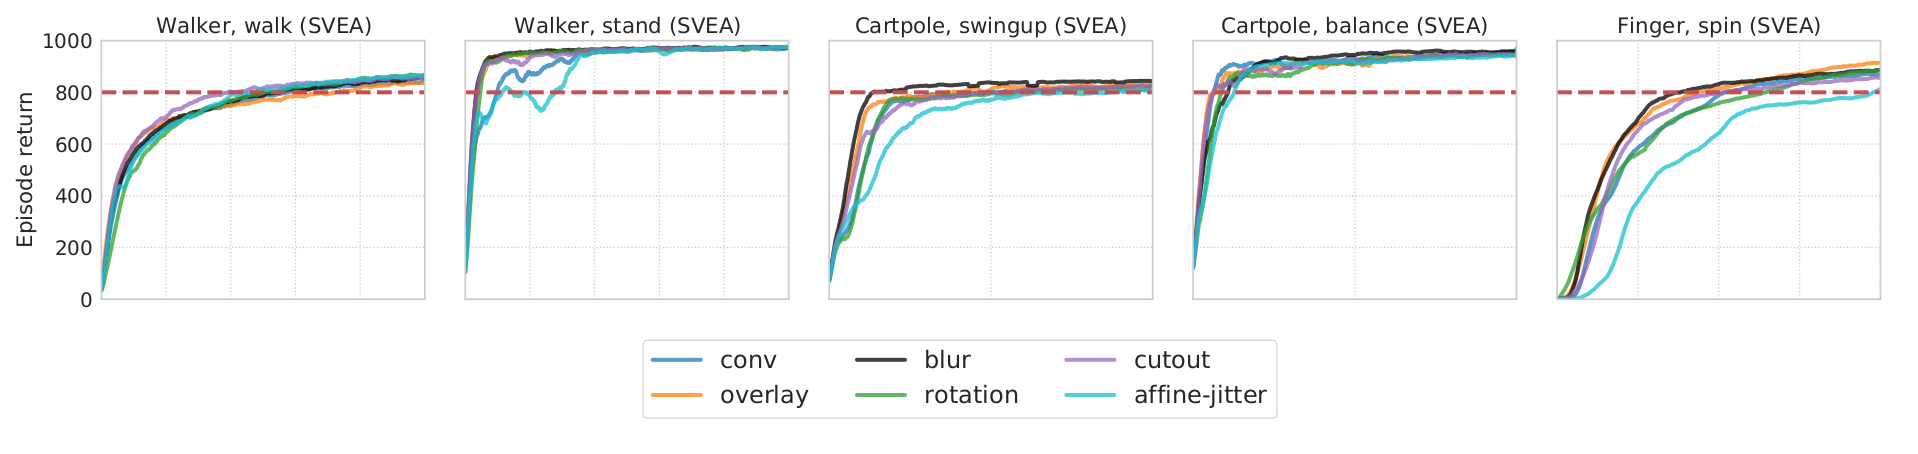
\includegraphics[width=\textwidth]{figures/drq_augs.png}
    \vspace{-0.2in}
    \caption{\textbf{Data augmentations.} Training performance of SVEA under 6 common data augmentations. Mean of 5 seeds. Red line at $800$ return is for visual guidance only. We omit visualization of std. deviations for clarity, but provide per-augmentation comparisons to DrQ (including std. deviations) across all tasks in Figure \ref{fig:drq-augs-suppl}, and test performances in Figure \ref{fig:data-aug-visualization}.}
    \label{fig:dmc-augs}
    \vspace{-0.125in}
\end{figure}
\begin{figure}[H]
    \centering
    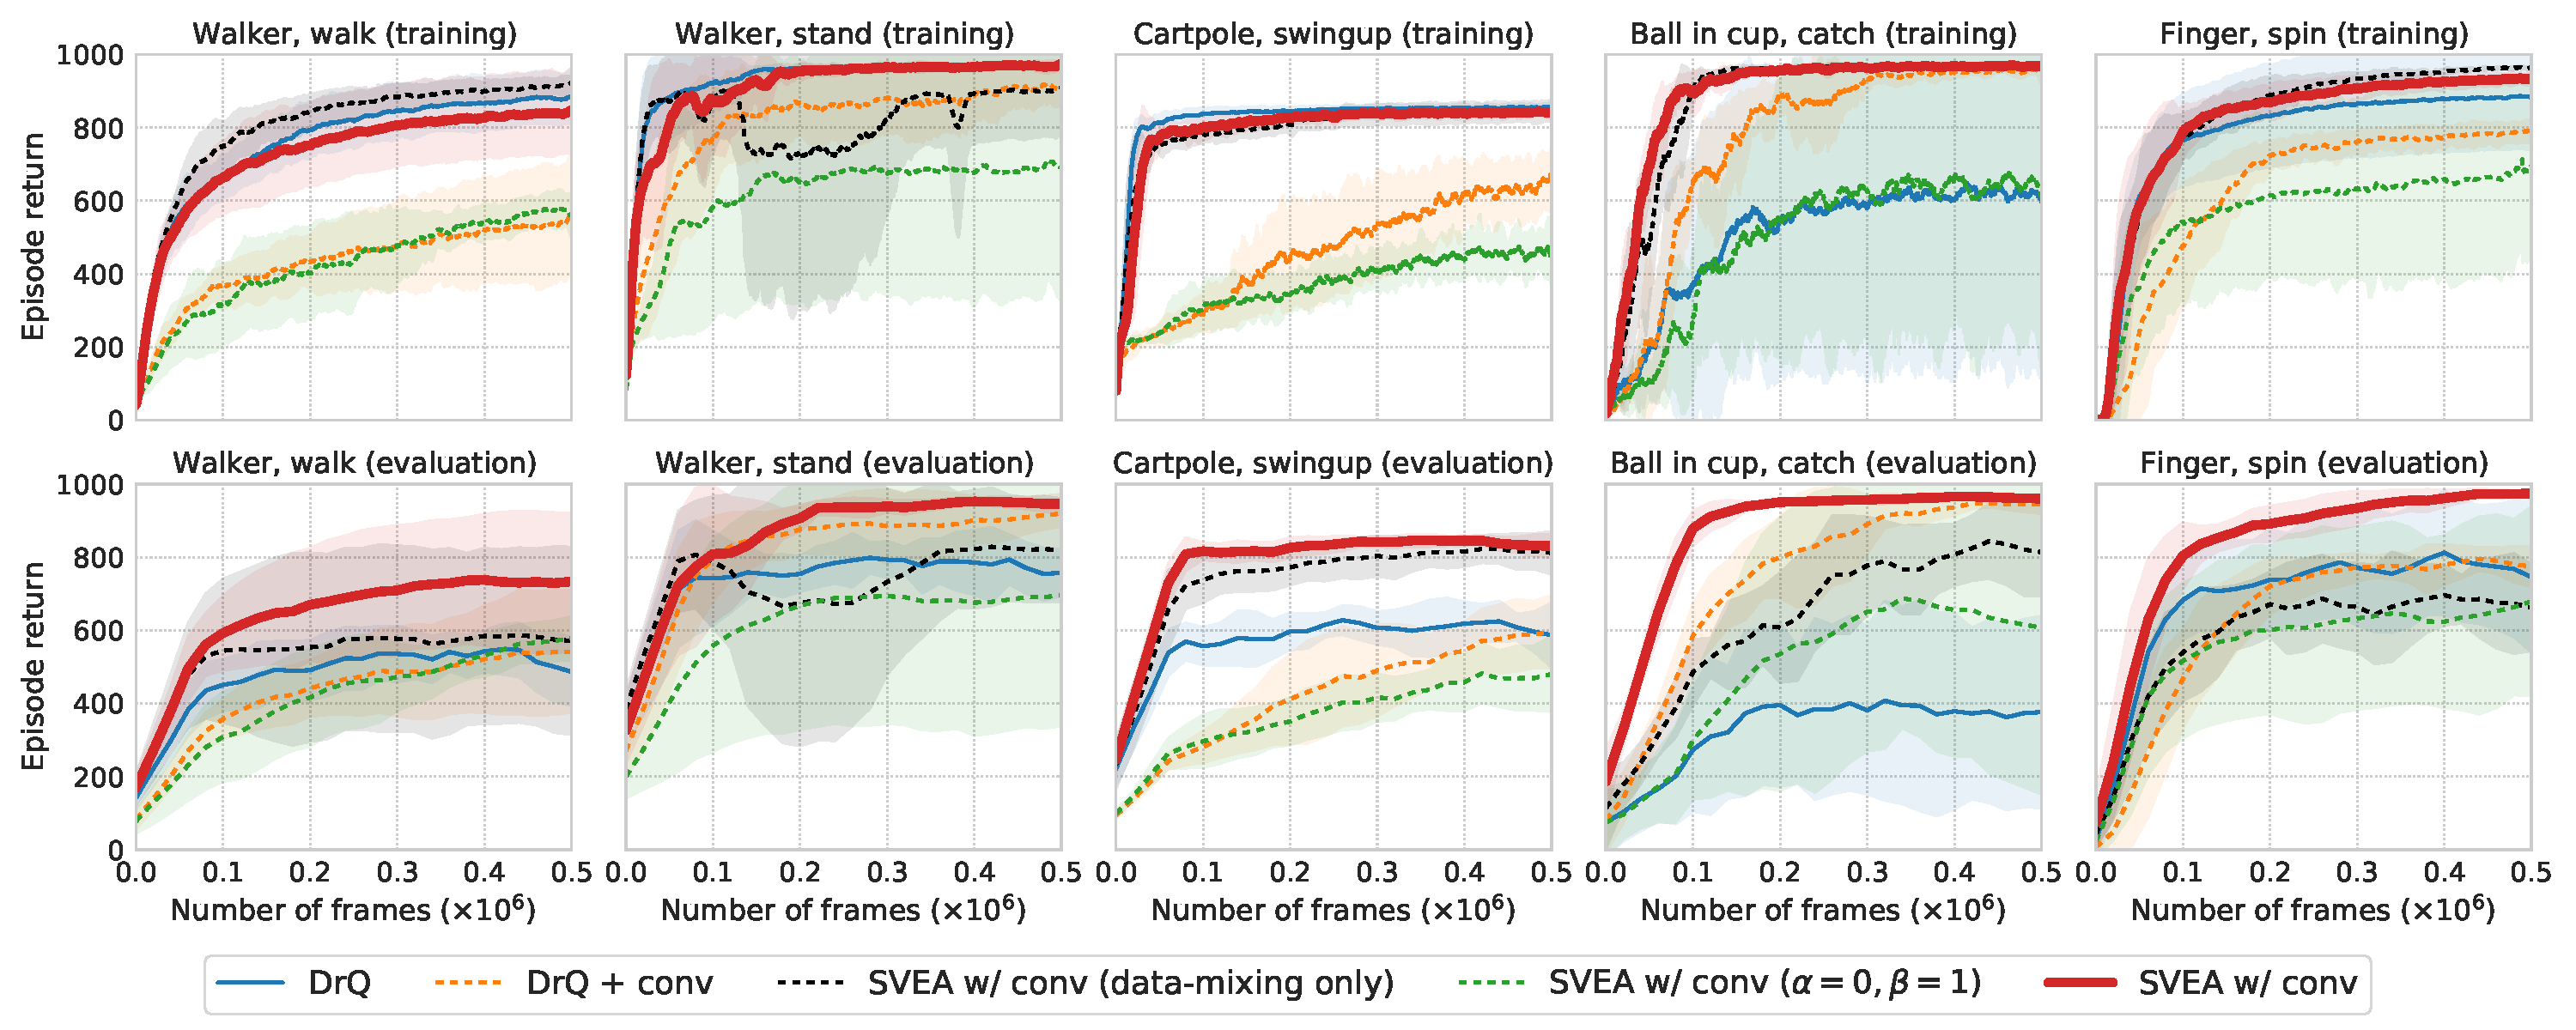
\includegraphics[width=\textwidth]{figures/drq_conv.pdf}
    \vspace{-0.2in}
    \caption{\textbf{Training and test performance.} We compare SVEA to DrQ with and without random convolution augmentation, as well as a set of ablations. \textit{Data-mixing only} indiscriminately applies our data-mixing strategy to all data streams, and $(\alpha=0, \beta=1)$ only augments $Q$-predictions but without data-mixing. We find both components to contribute to SVEA's success. \textit{Top:} episode return on the training environment during training. \textit{Bottom:} generalization measured by episode return on the \texttt{color\_hard} benchmark of DMControl-GB. Mean of 5 seeds, shaded area is $\pm1$ std. deviation.}
    \label{fig:dmc-conv}
    \vspace{-0.125in}
\end{figure}\\

\subsubsection*{\textbf{Stability under data augmentation}}
\label{sec:stability-under-data-augmentation}

Figure \ref{fig:drq-augs-suppl} compares the sample efficiency and stability of SVEA and DrQ under each of the 6 considered data augmentations for 5 tasks from DMControl. Stability of DrQ under data augmentation is found to be highly sensitive to both the choice of augmentation and the particular task. For example, the \textit{DrQ + aug} baseline is relatively unaffected by a majority of data augmentations in the \textit{Walker}, \textit{stand} task, while we observe significant instability across all data augmentations in the \textit{Cartpole}, \textit{swingup} task. Our results therefore indicate that SVEA can be a highly effective method for eliminating the need for costly trial-and-error associated with application of data augmentation.
\begin{figure}[H]
    \centering
    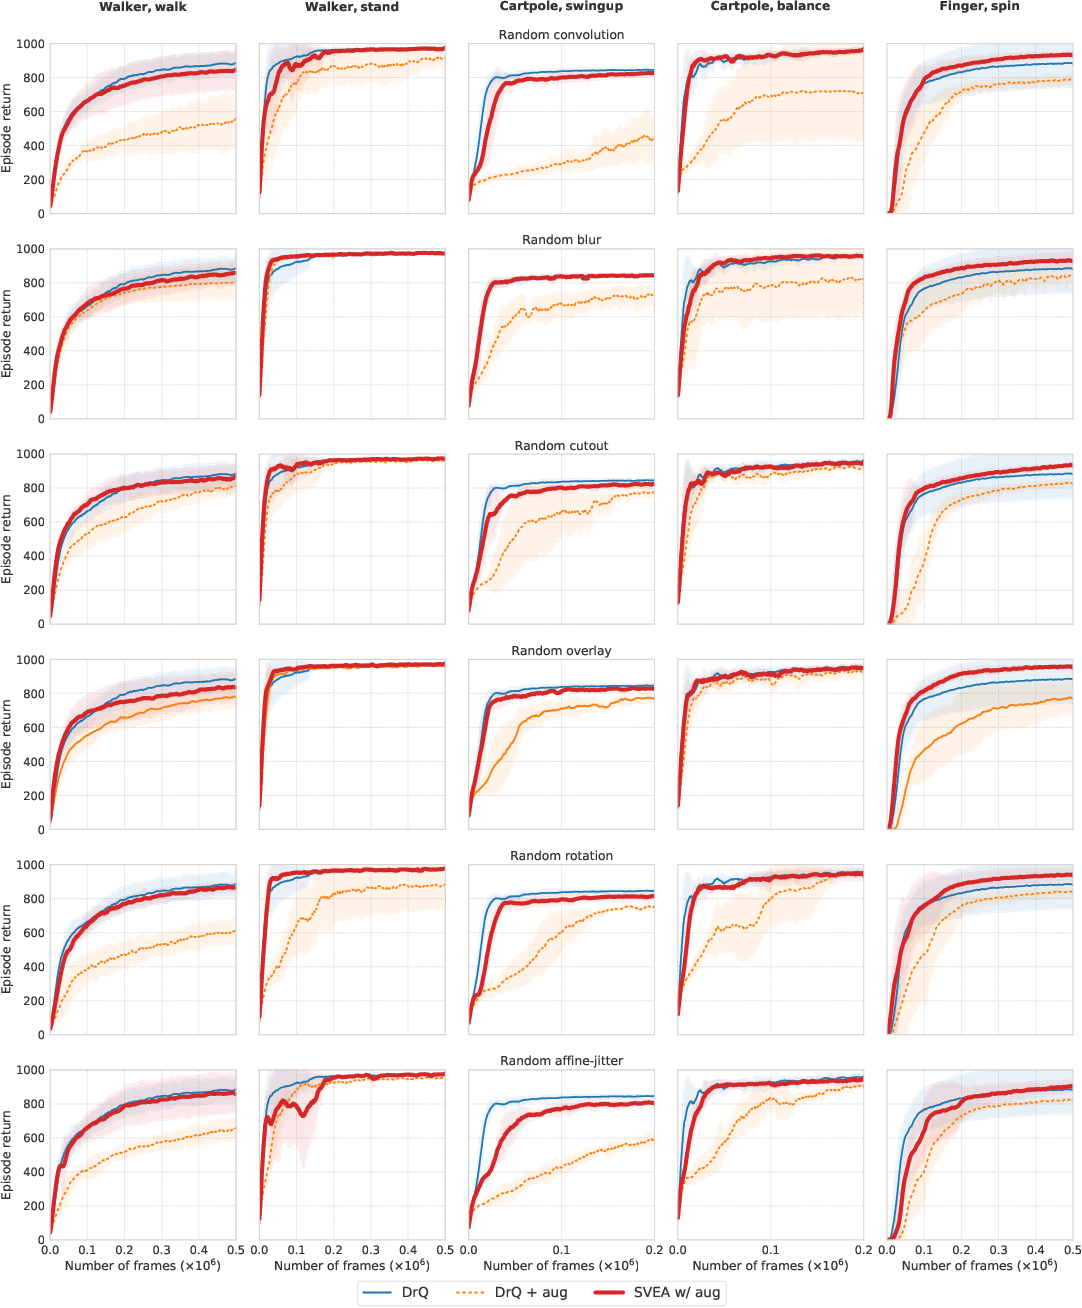
\includegraphics[width=\textwidth]{figures/drq_augs_suppl.png}
    \caption{\textbf{Stability under data augmentation.} Training performance measured by episode return of SVEA and DrQ under 6 common data augmentations (using ConvNets). We additionally provide reference curves for DrQ without additional augmentation. Mean of 5 seeds, shaded area is $\pm1$ std. deviation. SVEA obtains similar sample efficiency to DrQ without augmentation, while the sample efficiency of \textit{DrQ + aug} is highly dependent on the task and choice of augmentation.}
    \label{fig:drq-augs-suppl}
    \vspace{-0.1in}
\end{figure}

%----------------------------------------------------------------------------------------
%	Section 5
%----------------------------------------------------------------------------------------

\subsection{\textbf{Generalization.}}
Here the test performance of SVEA is compared to 5 recent state-of-the-art methods for image-based RL on the \texttt{color\_hard} and \texttt{video\_easy} benchmarks from DMControl-GB, as well as the extremely challenging DistractingCS benchmark, where camera pose, background, and colors are continually changing throughout an episode. Here \textit{conv} and \textit{overlay} augmentations are used and we report additional results on the \texttt{video\_hard} benchmark. SVEA outperforms all methods considered in $\mathbf{12}$ out of $\mathbf{15}$ instances on DMControl-GB, and at a lower computational cost than CURL, PAD, and SODA that all learn auxiliary tasks. On DistractingCS, we observe that SVEA improves generalization by $\mathbf{42\%}$ at low intensity, and its generalization degrades significantly slower than DrQ for high intensities. While generalization depends on the particular choice of data augmentation and test environments, this is an encouraging result considering that SVEA enables efficient policy learning with stronger augmentations than previous methods.


\subsection{\textbf{Test Environments}}
Figure \ref{fig:test-env-visualization} provides visualizations for each of the two generalization benchmarks, DMControl Generalization Benchmark and Distracting Control Suite, used in our experiments. Agents are trained in a fixed training environment with no visual variation, and are expected to generalize to novel environments of varying difficulty and factors of variation. The \texttt{color\_hard}, \texttt{video\_easy}, and \texttt{video\_hard} benchmarks are from DMControl Generalization Benchmark, and we further provide samples from the Distracting Control Suite (DistractingCS) benchmark for intensities $I=\{0.1, 0.2, 0.5\}$. 
While methods are evaluated on a larger set of intensities, we here provide samples deemed representative of the intensity scale. We note that the DistractingCS benchmark has been modified to account for action repeat (frame-skip). Dynamically changing the environment at each simulation step makes the benchmark disproportionally harder for tasks that use a large action repeat, e.g. \textit{Cartpole} tasks. Therefore, we choose to modify the DistractingCS benchmark and instead update the distractors every second simulation step, corresponding to the lowest action repeat used (2, in \textit{Finger, spin}). This change affects both SVEA and baselines equally. Figure \ref{fig:dmc-dcs-individual} shows generalization results on DistractingCS for each task individually. We find that the difficulty of DistractingCS varies greatly between tasks, but SVEA consistently outperforms DrQ in terms of generalization across all intensities and tasks.

\begin{figure}
    \centering
    \begin{subfigure}[b]{0.48\textwidth}
        \centering
        
\includegraphics[width=\textwidth]{figures/visualizations/obs_env.png}
        \caption{Training environment (walker).}
        \vspace{0.1in}
    \end{subfigure}
    \begin{subfigure}[b]{0.48\textwidth}
        \centering
        
\includegraphics[width=\textwidth]{figures/visualizations/obs_cartpole_env.png}
        \caption{Training environment (cartpole).}
        \vspace{0.1in}
    \end{subfigure}
    \begin{subfigure}[b]{0.48\textwidth}
        \centering
        
\includegraphics[width=\textwidth]{figures/visualizations/obs_env_color_hard.png}
        \caption{\texttt{color\_hard} environment (walker).}
        \vspace{0.1in}
    \end{subfigure}
    \begin{subfigure}[b]{0.48\textwidth}
        \centering
        
\includegraphics[width=\textwidth]{figures/visualizations/obs_cartpole_env_color_hard.png}
        \caption{\texttt{color\_hard} environment (cartpole).}
        \vspace{0.1in}
    \end{subfigure}
    \begin{subfigure}[b]{0.48\textwidth}
        \centering
        
\includegraphics[width=\textwidth]{figures/visualizations/obs_env_video_easy.png}
        \caption{\texttt{video\_easy} environment (walker).}
        \vspace{0.1in}
    \end{subfigure}
    \begin{subfigure}[b]{0.48\textwidth}
        \centering
        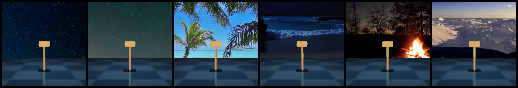
\includegraphics[width=\textwidth]{figures/visualizations/obs_cartpole_env_video_easy.png}
        \caption{\texttt{video\_easy} environment (cartpole).}
        \vspace{0.1in}
    \end{subfigure}
    \begin{subfigure}[b]{0.48\textwidth}
        \centering
        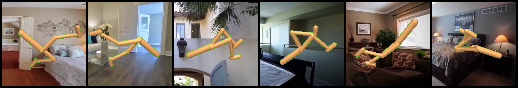
\includegraphics[width=\textwidth]{figures/visualizations/obs_env_video_hard.png}
        \caption{\texttt{video\_hard} environment (walker).}
        \vspace{0.1in}
    \end{subfigure}
    \begin{subfigure}[b]{0.48\textwidth}
        \centering
        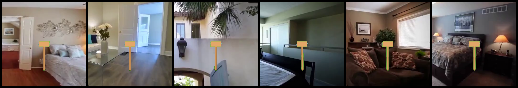
\includegraphics[width=\textwidth]{figures/visualizations/obs_cartpole_env_video_hard.png}
        \caption{\texttt{video\_hard} environment (cartpole).}
        \vspace{0.1in}
    \end{subfigure}
    \begin{subfigure}[b]{0.48\textwidth}
        \centering
        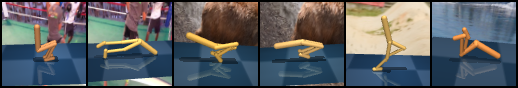
\includegraphics[width=\textwidth]{figures/visualizations/obs_env_dcs_easy.png}
        \caption{DistractingCS for intensity $0.1$ (walker).}
        \vspace{0.1in}
    \end{subfigure}
    \begin{subfigure}[b]{0.48\textwidth}
        \centering
        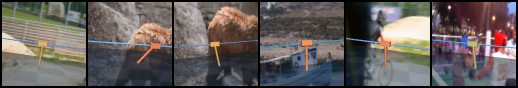
\includegraphics[width=\textwidth]{figures/visualizations/obs_cartpole_env_dcs_easy.png}
        \caption{DistractingCS for intensity $0.1$ (cartpole).}
        \vspace{0.1in}
    \end{subfigure}
    \begin{subfigure}[b]{0.48\textwidth}
        \centering
        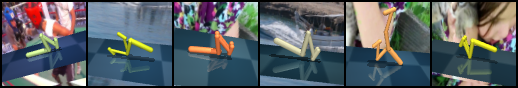
\includegraphics[width=\textwidth]{figures/visualizations/obs_env_dcs_medium.png}
        \caption{DistractingCS for intensity $0.2$ (walker).}
        \vspace{0.1in}
    \end{subfigure}
    \begin{subfigure}[b]{0.48\textwidth}
        \centering
        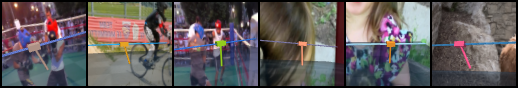
\includegraphics[width=\textwidth]{figures/visualizations/obs_cartpole_env_dcs_medium.png}
        \caption{DistractingCS for intensity $0.2$ (cartpole).}
        \vspace{0.1in}
    \end{subfigure}
    \begin{subfigure}[b]{0.48\textwidth}
        \centering
        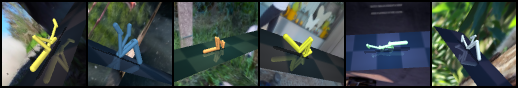
\includegraphics[width=\textwidth]{figures/visualizations/obs_env_dcs_extreme.png}
        \caption{DistractingCS for intensity $0.5$ (walker).}
        \vspace{0.1in}
    \end{subfigure}
    \begin{subfigure}[b]{0.48\textwidth}
        \centering
        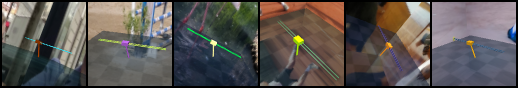
\includegraphics[width=\textwidth]{figures/visualizations/obs_cartpole_env_dcs_extreme.png}
        \caption{DistractingCS for intensity $0.5$ (cartpole).}
        \vspace{0.1in}
    \end{subfigure}
    \vspace{-0.1in}
    \caption{\textbf{Test environments}. Samples from each of the two generalization benchmarks, DMControl Generalization Benchmark and Distracting Control Suite, considered in this study. In our experiments, agents are trained in a fixed training environment with no visual variation, and are expected to generalize to novel environments of varying difficulty and factors of variation.}
    \label{fig:test-env-visualization}
    \vspace{-0.15in}
\end{figure}

\begin{figure}
    \centering
    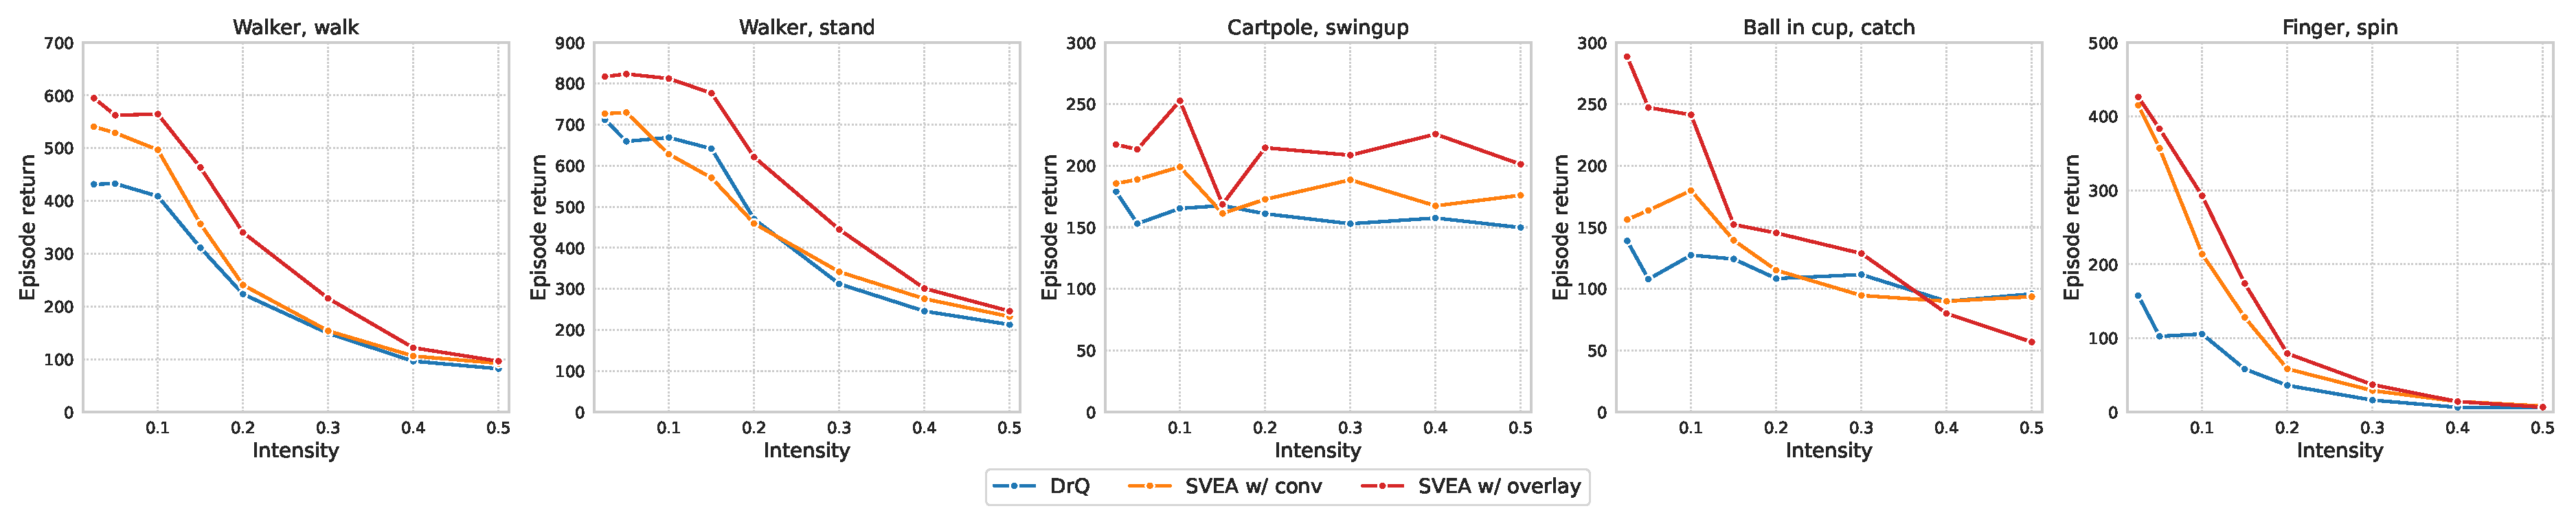
\includegraphics[width=\textwidth]{figures/dcs_individual.pdf}
    \vspace{-0.2in}
    \caption{\textbf{DistractingCS.} Episode return as a function of randomization intensity, for each of the 5 tasks from DMControl-GB (using ConvNets). Mean of 5 seeds. We find that the difficulty of DistractingCS varies greatly between tasks, but SVEA consistently outperforms DrQ in terms of generalization across all intensities and tasks, except for \textit{Ball in cup, catch} at the highest intensity.}
    \label{fig:dmc-dcs-individual}
    \vspace{-0.05in}
\end{figure}

%----------------------------------------------------------------------------------------
%	Section 6
%----------------------------------------------------------------------------------------

\newpage
\section{My Experiments}

When exploring enhancements for SVEA, there are several factors to consider. Given the limitations imposed by hardware, we need to scale our suggestions to align with the available GPUs provided by Google Collaboratory. Within this context, we focus on two aspects of the problem formulation:
\begin{enumerate}
    \item Introducing non-determinism in the test environment. This entails considering how this change should be reflected in the applied data augmentations.
    
    \item Analyzing the relationship between adjustments made to the test domain's parameters and the corresponding modifications required for data augmentation parameters. 
\end{enumerate}

\subsection{Non-Determinism}
Training an RL algorithm for continuous control tasks in a deterministic environment can simplify the learning process as the agent can directly associate actions with specific outcomes. However, there are a few considerations to keep in mind. First, deterministic environments may not fully capture the complexity and uncertainty of real-world scenarios. If the goal is to develop RL algorithms that can generalize to uncertain or stochastic environments, training solely in a deterministic environment may limit the algorithm's ability to adapt to such conditions.
Ultimately, in some cases, training in a deterministic environment may result in the agent overfitting to that specific environment. The learned policy may not generalize well to different variations or perturbations of the environment. To address this, it can be beneficial to introduce randomization or variability during training, such as through the use of stochastic dynamics or adding noise to the actions or observations.

The DMControl environments are, in fact, deterministic by default. To make them non-deterministic, you can introduce stochasticity into the environments by adding random factors. Here's how you can achieve this:
\begin{itemize}
    \item \textbf{Perturb the dynamics:} You can introduce random noise or variations in the dynamics of the environment. This can be done by modifying the physics parameters, such as friction, mass, or joint constraints, with random values.

    \item \textbf{Add sensory noise:} Introduce random noise to the observations received by the agent. This can simulate uncertainty or variability in the sensor measurements.

    \item \textbf{Randomize initial conditions:} Vary the initial states of the environment to provide different starting points for each episode. This can be done by sampling initial positions, velocities, or other relevant variables from a distribution.

    \item \textbf{Modify reward functions:} Randomize or introduce stochasticity in the rewards given to the agent. This can create variability in the feedback received and affect the agent's behavior.
    
\end{itemize}


By applying these techniques, we can introduce non-determinism into the DMControl environments, making them more realistic and challenging for reinforcement learning algorithms.

In DM Control Suite we have the following parameters that can be used for this purpose:
\begin{itemize}
    \item $random$: Optional, either a `numpy.random.RandomState` instance, an integer
        seed for creating a new `RandomState`, or None to select a seed automatically (default).
\end{itemize}
We can choose the same seed for the training environment and the testing environment and therefore we will have a non-deterministic test environment.


\subsection{Adjusting the augmentations}
The application of weak augmentation, such as random shift, has been shown to improve sample efficiency without causing significant issues. However, it has been observed that strong augmentation, such as random convolution, can lead to instability and poor sample efficiency. The use of stronger and more varied augmentations, including random convolution, random overlay, and affine-jitter, has the potential to enhance generalization to a broader range of Markov Decision Processes (MDPs). 
In SVEA, we add random convolution to make the augmented image. Here we will attempt to use random overlay alongside random convolution.

\newpage
% %bibliography
\bibliographystyle{unsrt}
\bibliography{sample.bib}

\end{document}